\chapter{The Compost Bomb and the Terrestrial Carbon Cycle}
\label{chapter:global_bomb}
\graphicspath{{global_bomb/figs/}}

\todo[inline]{This is basically just going to be equations for now}

In \cref{chapter:continuous_compost_bomb}, I introduced a vertical dimension into a model of the compost bomb. It was shown that this doesn't
surpress the compost bomb. That analysis was local ---  the modeling was done at a single point on the Earth's surface. It would be interesting to see
what a globally-averaged model that included biogeochemical heating would predict. Work by~\cite{Cox2006} suggested that the terrestrial carbon cycle is stable
only for certain parameter ranges. I will begin by investigating what effect biogeochemical heating has on this.

\section{Compost Bomb Bifurcation Analysis}

\subsection{Dynamical Equations}
The compsot bomb equations, introduced by~\cite{Luke2011}, are
\begin{subequations}
  \label{eq:compost_bomb_equations}
  \begin{align}
    \mu \dv{T_s}{t} &= - \kappa \left(T_s - T_a\right) + Ar_0C_se^{\alpha T_s} \label{eq:compost_bomb_soil_temperature} \\
    \dv{C_s}{t} &= \Pi - r_0C_se^{\alpha T_s}, \label{eq:compost_bomb_soil_carbon}
  \end{align}
\end{subequations}
where $T_s$ and $C_s$ are soil temperature and carbon, $T_a$ is the atmospheric temperature, $\alpha = 0.1\log Q_{10}$ is the sensitivity of
temperature to respiration, $\Pi$ is Net Primary Productivity, $A$ is the heat released by respiration, $\kappa$ is a heat transfer coefficent,
$\mu$ is a heat capacity and $r_0$ is the specific rate of respiration.

While the analysis in~\cite{Luke2011} was local, it will be assumed that \cref{eq:compost_bomb_equations} hold at the global scale too, where quanities are
replaced by their global value. It will also be assumed that Net Primary Productivity, $\Pi$, is an increasing function of atmospheric \ce{CO2}, as is $T_a$. 

There is a timescale separation in \cref{eq:compost_bomb_equations}. The dynamic of soil carbon are relatively slow, with a soil turn over time measured in the decades \parencite{Varney2022},
whereas the dynamics of soil temperature are much faster, reaching an equilibrium with the air temperature on the time scale of a day \parencite{Best2005}. With this in mind, the soil
temperature can be set to equilibrium by setting \cref{eq:compost_bomb_soil_temperature} equal to zero. This gives
\begin{equation*}
  0 = - \kappa \left(T_s - T_a\right) + Ar_0C_se^{\alpha T_s}
\end{equation*}
which can be solved for the soil temperature to  give
\begin{equation}
  \label{eq:soil_temperature_equilibrium}
  T_s = T_a - \frac{1}{\alpha} W\left(-\frac{Ar_0C_s \alpha e^{\alpha T_a}}{\kappa} \right),
\end{equation}
where $W(x)$ is the Lambert $W$ function \parencite{Corless1996}. The Lambert $W$ function, plotted in \cref{fig:lambert_W}, is defined as the solution to the equation
\begin{equation}
  \label{eq:lambert_W}
  W(x)e^{W(x)} = x.
\end{equation}

\begin{figure}
  \centering
  \begin{tikzpicture}
    \begin{axis}[
      xmin=-1,
      xmax=4,
      enlarge y limits=false,
      axis lines=left,
      xlabel=$x$,
      ylabel=$W(x)$,
      samples=50]
      \addplot[domain=-5:-1] (x * exp(x), x);
      \addplot[domain=-1:2] (x * exp(x), x);
    \end{axis}
  \end{tikzpicture}
  \caption[The Lambert $W$ function]{The Lambert $W$ function, for $x \in [-1,4]$. The minimum value of $x$ for which $W$ is defined is $-1/e$. For $x < 0$, $W(x)$ is
  multivalued.}
  \label{fig:lambert_W}
\end{figure}
\todo{This figure should have conventionally positioned axes}

After noting that the argument of $W$ should be dimensionless, and that $r_0C_s$ has units of Net Primary Productivity, the quantity 
\begin{equation}
  \label{eq:critical_npp}
  \Pi_c = \frac{\kappa}{\alpha A}
\end{equation}
can be defined, which measures the influence of biogeochemical heating. No biogeochemical heating occurs for $A = 0$ or equivalently $\Pi_c = \infty$. Similarly
biogeochemical heating is strongest for $A \rightarrow \infty$ or again equivalently fpr $\Pi_c = 0$.

\Cref{eq:soil_temperature_equilibrium} can now be rewritten as
\begin{equation}
  \label{eq:soil_temperature_equilibrium_nppc}
  T_s = T_a - \frac{1}{\alpha} W\left(-\frac{r_0C_s e^{\alpha T_a}}{\Pi_c} \right).
\end{equation}
\Cref{eq:soil_temperature_equilibrium_nppc} can now be inserted into \cref{eq:compost_bomb_soil_carbon} to give
\begin{equation}
  \label{eq:soil_carbon_evolution}
  \dv{C_s}{t} = \Pi + \Pi_c W\left(-\frac{r_0C_s e^{\alpha T_a}}{\Pi_c} \right).
\end{equation}
which for given $\Pi$ and $T_a$ determines the evolution of $C_s$.

The implied equilibrium value for $C_s$ occurs when \cref{eq:soil_carbon_evolution} is zero which occurs when
\begin{equation}
  \label{eq:equilibirum_soil_carbon}
  C_s^{\mathrm{eq}} = \frac{\Pi}{r_0} e^{-\alpha T_a} e^{-\Pi/\Pi_c}.
\end{equation}
The no biogeochemcial heating case can be recovered by sending $\Pi_c \rightarrow \infty$ which gives $C_s^{\mathrm{eq}} = \frac{\Pi}{r_0}$.

\subsection{Closing the System}
It has been stated that $T_a$ and $\Pi$ are functions of atmospheric carbon, so to determine their behaviours requires specifying the behaviour of the rest of the carbon
cycle. The total carbon in the carbon cycle is conserved and so
\begin{equation}
  \label{eq:carbon_conservation}
  C_s + C_a + C_o = C_s^{\mathrm{eq}} + C_{a0} + C_{o0}
\end{equation}
where $C_a$ and $C_o$ are atmospheric and oceanic carbon and the quanitities on the righthand side are the equilibrium values.
Following~\cite{Cox2006}, it will be assumed that a fixed fraction, $\chi_0$, of atmospheric emissions reaches the ocean, meaning
\begin{equation}
  \label{eq:simple_ocean}
  C_a = C_{a0} -\frac{1}{1+\chi_0} (C_s - C_{s}^{\mathrm{eq}}).
  %C_s = C_{s}^{\mathrm{eq}} - (1 + \chi_0)(C_a - C_{a0}.
\end{equation}

Making the further assumption that atmospheric temperatures scale logarithmically with atmospheric \ce{CO2} \parencite{Pierrehumbert2010} gives
\begin{equation}
  \label{eq:atmospheric_temperatures}
  T_a = \frac{S}{\log 2} \log \frac{C_a}{C_{a0}} 
\end{equation}
where $S$ is the effective climate sensitivity experienced by the soils. Substituting \cref{eq:atmospheric_temperatures} into \cref{eq:soil_carbon_evolution} 
leads to
\begin{equation}
  \label{eq:global_soil_carbon}
  \dv{C_s}{t} = \Pi(C_a) + \Pi_c W\left(-\frac{r_0C_s}{\Pi_c} \left(\frac{C_a}{C_{a0}}\right)^\mu \right),
\end{equation}
where
\begin{equation}
  \label{eq:mu}
  \mu = \frac{\alpha S}{\log 2}
\end{equation}
and $C_a$ is determined through \cref{eq:simple_ocean}. By assumption, $C_s = C_s^{\mathrm{eq}}$ when $T_a = 0$ which means that 
$r_0 = \frac{\Pi_0}{C_s^{\mathrm{eq}}}e^{-\Pi_0/\Pi_c}$, where $\Pi_0 = \Pi\left(C_{a0}\right)$.

To numerically compute the equilibria of \cref{eq:global_soil_carbon}, the dependence of $\Pi$ on
$C_a$  must be set. It is chosen to be
\begin{equation}
  \label{eq:npp_fertilization}
  \Pi(C_a) = \frac{\Pi_{\infty} C_a}{C_a + C_{a_{1/2}}}.
\end{equation}
This is an increasing function of $C_a$, which saturates to $\Pi_{\infty}$ for $C_a \gg C_{a_{1/2}}$.

It is now straightforward to compute the bifurcation diagram, which is plotted in \cref{fig:compost_bomb_bif}.
\begin{figure}
  \centering
  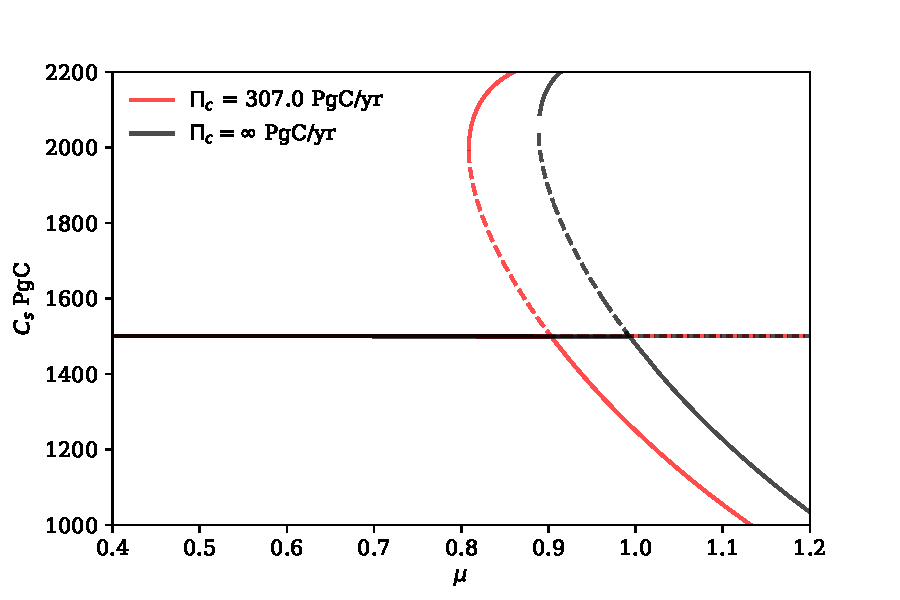
\includegraphics[width=\textwidth,keepaspectratio]{compost_bomb_global_bifurcation}
  \caption[Global Compost Bomb Bifurcation Diagram]{The equilibrium state of \cref{eq:global_soil_carbon} for two values of $\Pi_c$ as a function of $\mu$.
    The two values of $\Pi_c$ represent a no biogeochemical heating case ($\Pi_c = \infty$) and a biogeochemical heating case ($\Pi_c = \SI{308}{\peta\gram\carbon\per\year}$).
    The other parameters were set to $\chi_0 = 0.25$, $\Pi_0 =\SI{55}{\peta\gram\carbon\per\year}$, $C_{1/2} = \SI{593.6}{\peta\gram\carbon}$, $C_{a0} = \SI{589}{\peta\gram\carbon}$,
  $C_{s}^{\mathrm{eq}} = \SI{1500}{\peta\gram\carbon}$.}
  \label{fig:compost_bomb_bif}
\end{figure}

\subsection{Computation of Bifurcation Point}
We can make analytic progress too. To find the bifurcation we therefore just have to calculate where
\begin{equation*}
  \dv{\dot{C_s}}{C_s} = 0,
\end{equation*}
we will make use of
\begin{equation}
  \label{eq:derivative_of_lambert_W}
  W'(x) = \frac{W(x)}{x\left(1 + W\left(x\right)\right)}.
\end{equation}




Taking a derivative of the right hand side of \cref{eq:global_soil_carbon} and setting it to zero in equilibrium gives
\begin{equation}
  \label{eq:soil_carbon_lambda}
  \dv{\Pi}{C_a}\dv{C_a}{C_s} + \frac{\Pi_c}{C_s^{\mathrm{eq}}} \frac{W\left(-\frac{r_0C_s^{\mathrm{eq}}}{\Pi_c}\right)}{1+W\left(-\frac{r_0C_s^{\mathrm{eq}}}{\Pi_c}\right)} \left(
    1 + \mu \frac{C_s^{\mathrm{eq}}}{C_{a0}} \dv{C_a}{C_s}\right) = 0
\end{equation}
so
\begin{equation}
  \label{eq:critical_mu}
  \mu = -\frac{C_{a0}}{C_{s}^{\mathrm{eq}}}\dv{C_s}{C_a}\left(\dv{\Pi}{C_a}\dv{C_a}{C_s} \frac{C_s^{\mathrm{eq}}}{\Pi_c}\frac{1+W\left(-\frac{r_0C_s^{\mathrm{eq}}}{\Pi_c}\right)}{W\left(-\frac{r_0C_s^{\mathrm{eq}}}{\Pi_c}\right)} + 1 \right)
\end{equation}
which simplifies to
\begin{equation}
  \label{eq:critical_mu_simple_ocean}
  \mu = \left(1+\chi_0\right) \frac{C_{a0}}{C_{s}^{\mathrm{eq}}} -
  \frac{C_{a0}}{\Pi_c}\frac{1+W\left(-\frac{r_0C_s^{\mathrm{eq}}}{\Pi_c}\right)}{W\left(-\frac{r_0C_s^{\mathrm{eq}}}{\Pi_c}\right)}\dv{\Pi}{C_a}.
\end{equation}
This can be further reduced to
\begin{equation*}
  \mu = \left(1+\chi_0\right) \frac{C_{a0}}{C_{s}^{\mathrm{eq}}} -
  \frac{C_{a0}}{\Pi_c}
  \frac{1+W\left(-\frac{\Pi_0}{\Pi_c}\exp\left(-\frac{\Pi_0}{\Pi_c}\right)\right)}
  {W\left(-\frac{\Pi_0}{\Pi_c}\exp\left(-\frac{\Pi_0}{\Pi_c}\right)\right)}\dv{\Pi}{C_a} 
\end{equation*}
and even more to give
\begin{equation*}
  \mu = \left(1+\chi_0\right) \frac{C_{a0}}{C_{s}^{\mathrm{eq}}} -
  \frac{C_{a0}}{\Pi_c}
  \frac{1-\frac{\Pi_0}{\Pi_c}}{-\frac{\Pi_0}{\Pi_c}}\dv{\Pi}{C_a}.
\end{equation*}
Cleaning this up gives the final form.
\begin{equation}
  \label{eq:critical_mu_simple_ocean_in_terms_of_npp}
  \mu^* = \left(1+\chi_0\right) \frac{C_{a0}}{C_{s}^{\mathrm{eq}}} +
  \frac{C_{a0}}{\Pi_0} \dv{\Pi}{C_a} - \frac{C_{a0}}{\Pi_c}\dv{\Pi}{C_a}.
\end{equation}
We remark that taking the limit where $\Pi_c \rightarrow \infty$ gives
\begin{equation}
  \label{eq:mu_infinity}
  \mu^*_{\infty} =\left(1+\chi_0\right) \frac{C_{a0}}{C_{s}^{\mathrm{eq}}} +
  \frac{C_{a0}}{\Pi_0} \dv{\Pi}{C_a}.
\end{equation}
This corresponds to the limit where biogeochemcial heating does not occur.

% We note this implies a minimum allowed \ce{CO2} fertilization effect for a given $\mu$ (as we need $\mu < \mu_\infty^*$)
% \begin{equation}
%   \label{eq:minimum_allowed_co2_fertilization}
%   \dv{\Pi}{C_a} > \frac{\Pi_0\mu}{C_{a0}} - \frac{1+\chi_0}{C_s^{\mathrm{eq}}}\Pi_0
% \end{equation}


We can plot \cref{eq:critical_mu} to devide the parameter plane into a stable and unstable region.

\begin{figure}
  \centering
  \begin{tikzpicture}[
    /pgf/declare function={
      chi0 = 0.25;
      npp = 55.0;
      Ca0 = 589.0;
      Cseq = 1500.0;
    }
    ]
    \begin{axis}[
      legend pos=outer north east,
      % enlargelimits=false
      xlabel={$\Pi_c$},
      ylabel={$\mu$},
      xmin=20,
      xmax=500,
      ymin=0.0
      ]
      \addplot[
      domain=20:500,
      samples=100,
      color=red]
      {(1+chi0)*Ca0/Cseq + 0.07 * ((Ca0/npp)  - (Ca0/x))};
      \addplot[
      domain=20:500,
      samples=100,
      color=red,
      dashed]
      {(1+chi0)*Ca0/Cseq + 0.07 * ((Ca0/npp))};
      \addlegendentry{$\dv*{\Pi}{C_a} = 0.07$}
    \end{axis}
  \end{tikzpicture}
  \caption{The parameter plane}
  \label{fig:critical_mu_vs_pic}
\end{figure}


\section{What is $S$?}
\todo[inline]{Can also look at respiration directly}
Ignoring the effects of biogeochemical heating, we can write spatially resolved soil carbon equations:
\begin{equation}
  \label{eq:spatially_resolved_soil_carbon}
  \pdv{C_s(\bm{r},t)}{t} = \Pi(\bm{r},t) - r_0(\bm{r},t)C_s(\bm{r},t)e^{\alpha T(\bm{r},t)}
\end{equation}
Averaging gives
\begin{equation}
  \label{eq:spatially_averaged_soil_carbon}
  \dv{\left\langle C_s\right\rangle}{t} = \left\langle \Pi \right \rangle - \left\langle r_0 C_s e^{\alpha T} \right \rangle
\end{equation}
Expanding:
\begin{align*}
  \dv{\left\langle C_s\right\rangle}{t} &\approx \left\langle \Pi \right \rangle - \left\langle r_0 C_s + r_0 C_s \alpha T \right \rangle \\
                                        &\approx \left\langle \Pi \right \rangle - \left\langle r_0 C_s\right \rangle - \alpha \left \langle r_0C_s T\right\rangle \\
                                        &=\approx - \alpha \left \langle \Pi T\right\rangle,
\end{align*}
where we have used $\Pi = r_0C_s$ in equilibrium. Introducting an effective temperature $T_{\mathrm{eff}}$ we get
\begin{equation*}
  - \alpha \left \langle \Pi T \right\rangle = - \alpha \left \langle \Pi \right\rangle T_{\mathrm{eff}}
\end{equation*}
so that
\begin{equation}
  \label{eq:definition_of_effective_temperature}
  T_{\mathrm{eff}} = \frac{\left \langle \Pi T \right\rangle}{\left \langle \Pi \right\rangle}.
\end{equation}
After a double of \ce{CO2} we have $T_{\mathrm{eff}} = S$ and $\langle T \rangle = \mathrm{ECS}$ so that
\begin{equation}
  \label{eq:S_vs_ECS}
  \frac{S}{\mathrm{ECS}} = \frac{\left \langle \Pi T \right\rangle}{\left \langle \Pi \right\rangle \left \langle T \right \rangle}.
\end{equation}
In words, $S$ is given by an NPP weighted average of global temperatures.
Based on HADGEM2-ES CMIP5 abrupt $4\times\ce{CO2}$ runs, we get $S/\mathrm{ECS} \approx 1.6$.
\section{What is $\Pi_c$?}
\todo[inline]{Do with Physically based --- with Penman Monteith - this is giving me a constraint on the ratio?}
To get a reasonable estimate of $\Pi_c$, we need $\alpha$, $A$ and $\kappa$. With a value of $Q_{10} \approx 2$, we find $\alpha \approx 0.03$.
We take $A$ from biochemistry to be \SI{3.9E7}{\joule\per\kilo\gram\carbon}. To estimate $\kappa$, we neglect biogeochemical heating
in \cref{eq:compost_bomb_soil_temperature} to get
\begin{equation}
  \label{eq:soil_temp_no_biogeo}
  \mu \dot{T_s} = -\kappa \left( T_s -T_a \right)
\end{equation}
and then move to the frequency domain by fourier transforming to get power spectrum of $T_s$ in terms of $T_a$
\begin{equation}
  \label{eq:power_spectrum_of_Ts}
  \left| \tilde{T}_s\left(\omega\right)\right|^2 = \frac{\kappa^2 \left| \tilde{T}_a\left(\omega\right)\right|^2}{\omega^2 \mu^2 + \kappa^2}.
    \end{equation}
Estimates of $\kappa$ and $\mu$ can therefore be extracted from timeseries of global $T_a$ and $T_s$ giving $\kappa$ to be \SI{0.27}{\watt\per\meter}\todo{check units}
and so $\Pi_c \approx$ \SI{300}{\kilo\gram\carbon\per\year}\todo{check}

\section{Variability and Autocorrelation}
\begin{figure}
  \centering
  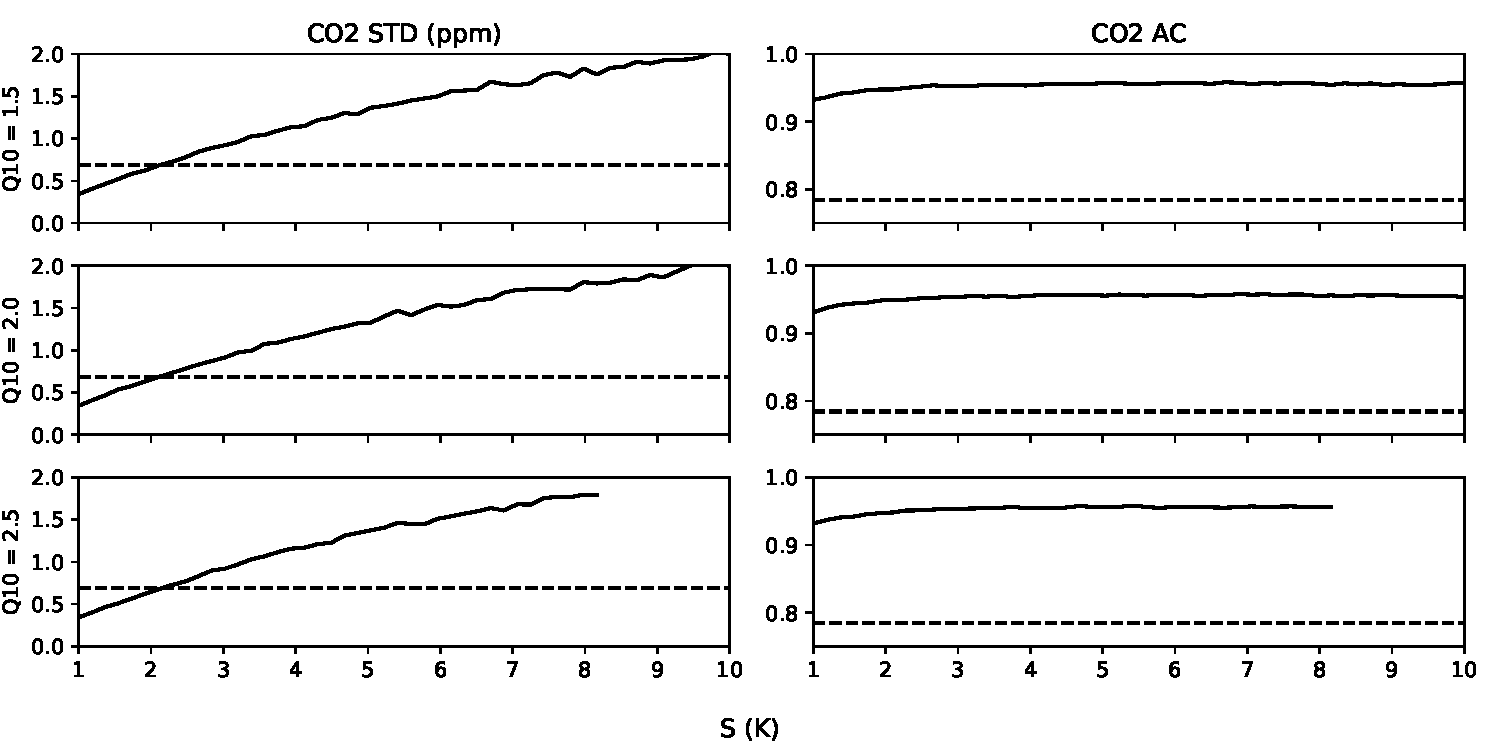
\includegraphics[width=\textwidth]{co2_std_ac}
  \caption[Atmospheric Carbon Variability]{Standard Deviation and Autocorrelation of atmospheric carbon}
  \label{fig:co2_std_ac}
  \end{figure}\todo{do this instead with more complex model}
  \begin{figure}
  \centering
  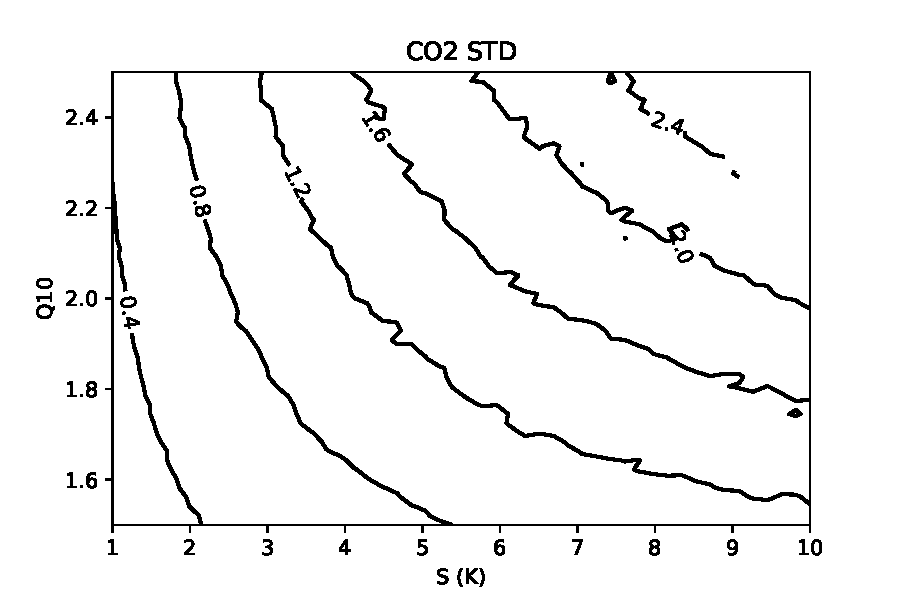
\includegraphics{co2stdcontour}
  \caption{CO2 standard deviation}
  \label{fig:co2_std_Q10_S}
\end{figure}
\begin{figure}
  \centering
  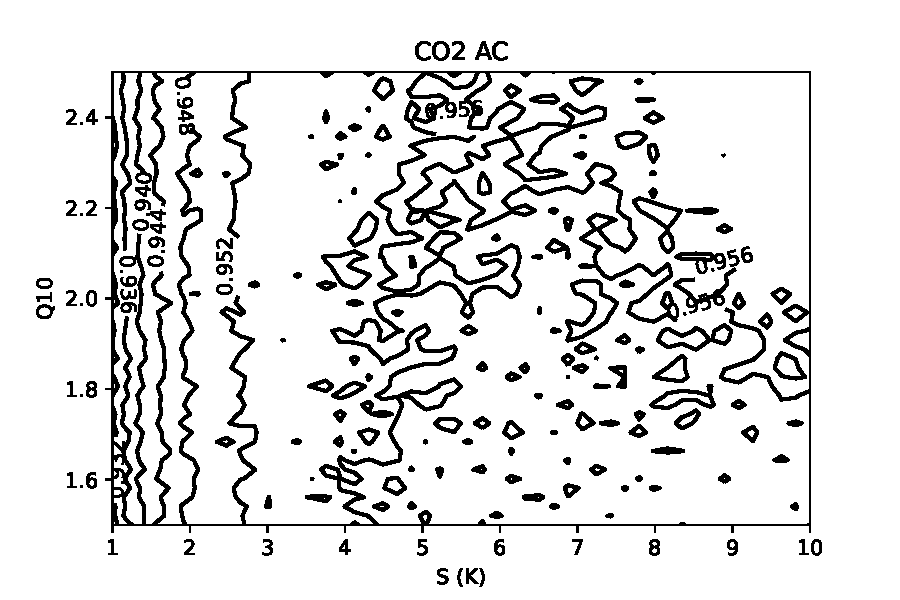
\includegraphics{co2accontour}
  \caption{CO2 AC}
  \label{fig:co2_ac_Q10_S}
\end{figure}